\section{Theorie}
\label{sec:Theorie}

\subsection{Versuchsziel}

Ziel des Versuches ist es, die Zeeman-Aufspaltung und Polarisation atomarer Spektrallinien
unter Einfluss eines äußeren Magnetfeldes zu untersuchen. Die Größe und Vielfalt 
der Aufspaltung werden für rote und blaue Cd-Spektrallinien der zugehörigen
optischen Übergänge analysiert.

\subsection{Elektrondrehimpulse und daran gekoppelte magnetische Momente}

Atomare Hüllenelektronen besitzen einen Bahndrehimpuls $\vec{l}$ und Spin $\vec{s}$
mit den zugehörigen Beträgen

\vspace{-25pt}
\begin{align}
    |\vec{l}| &= \hbar \sqrt{l(l+1)} & |\vec{s}| &= \hbar \sqrt{s(s+1)}
\end{align}

und Quantenzahlen $l$ und $s = \sfrac{1}{2}$. $l$ kann dabei abhängig von der Hauptquantenzahl $n$,
welche das Energieniveau der Elektronen angibt, ganzzahlige Werte zwischen $0$ und $n-1$ annehmen.
Über die Spin-Bahn-Kopplung können den Drehbewegungen der Elektronen die magnetischen Momente 

\vspace{-15pt}
\begin{align}
    \vec{\mu_l} &= - \frac{\mu_\text{B}}{\hbar} \cdot \vec{l}, & |\vec{\mu_l}|& = - \mu_\text{B} \sqrt{l(l+1)}\\
    \vec{\mu_s} &= - g_s \frac{\mu_\text{B}}{\hbar} \cdot \vec{s}, & |\vec{\mu_s}| &= - g_s \mu_\text{B} \sqrt{s(s+1)}
\end{align}

mit dem Bohrschen Magneton $\mu_B = -\frac{e_0 \hbar}{2 m_0}$ zugeordnet werden.
Der Landé-Faktor $g_s \approx 2$ beschreibt die magnetomechanische Anomalie des Elektrons.

\subsection{Verschiedene Drehimpulskopplungen}

\subsubsection{jj-Kopplung}

Die  jj-Kopplung dominiert in schweren Atomen hoher Ordnungszahl. 
Bahndrehimpulse $\l_i$ und Spin $\vec{s_i}$ der einzelnen Elektronen 
wechselwirken jeweils miteinander und ergeben die Gesamtdrehimpulse
 $\vec{j_i} = \vec{l_i} + \vec{s_i}$. Diese wechselwirken
 mit jenen anderer Elektronen und summieren sich zu einem
 Gesamtdrehimpuls der Elektronenhülle

\begin{equation}
    \vec{J} = \sum_i \vec{j_i} \; .
\end{equation}

\vspace{-20pt}
\subsubsection{LS-Kopplung}

Die LS-Kopplung hingegen dominiert in leichten Atomen niedriger Ordnungszahl
und ist daher von größerer Bedeutung für diesen Versuch.
In der Elektronenhülle wechselwirken im Gegensatz zur jj-Kopplung jeweils die Bahndrehimpulse $\vec{l_i}$
der Elektronen stärker untereinander und das gleiche gilt auch für die Spins $\vec{s_i}$.
Danach ergeben sich der Bahndrehimpuls $\vec{L}$ und der Spin $\vec{S}$
der gesamten Elektronenhülle als Summen der Einzelmomente zu

\begin{align}
    \qquad \vec{L} &= \sum_i \vec{l_i} \:, & |\vec{L}| = \hbar \sqrt{L(L+1)}\\
    \qquad \vec{S} &= \sum_i \vec{s_i} \:, & |\vec{S}| = \hbar \sqrt{S(S+1)}
\end{align}
\vspace{-10pt}

mit der ganzzahligen Quantenzahlen $L$ und $S$, wobei $S$ auch halbzahlig sein kann.  
An $\vec{L}$ und $\vec{S}$ koppeln die magnetischen Momente

\vspace{-15pt}
\begin{align}
 |\vec{\mu_L}|& = \mu_\text{B} \sqrt{L(L+1)} \:, &  |\vec{\mu_S}|& = g_S \mu_\text{B} \sqrt{S(S+1)}\: .
\end{align}

Der Gesamtdrehimpuls der Elektronenhülle ergibt sich schließlich zu

\vspace{-15pt}
\begin{align}
    \vec{J} &= \vec{L} + \vec{S} \:, & |\vec{J}| = \hbar \sqrt{J(J+1)} \: .
\end{align}

Die Quantenzahl $J$ ist abhängig von $S$ ganz- oder halbzahlig.
Dem Gesamtdrehipuls wird das magnetische Moment

\vspace{-15pt}
\begin{align}
    \vec{\mu_J} &= \vec{\mu_L} + \vec{\mu_S} \:, & |\vec{\mu_J}| = g_J \mu_\text{B} \sqrt{J(J+1)}
\end{align}

zugeordnet. Allerdings stimmen die Richtungen von $\vec{J}$ und $\vec{\mu_J}$ meist nicht überein und
nur die zu $\mu_J$ parallele $\vec{J}$-Komponente wird berücksichtigt - mit dem zugehörigen Landé-Faktor 

\begin{equation}
    g_J = \frac{3J(J+1) + S(S+1) - L(L+1)}{2J(J+1)}\: .
\end{equation}

\subsection{Zeeman-Aufspaltung im Magnetfeld}

Im äußeren Magnetfeld $\vec{B}$ ist eine Richtungsquantisierung des magnetischen Moments
$\mu_J$ zu beobachten, welche durch die ganzzahlige magnetische Quantenzahl $m$ beschrieben wird.
Die Komponente $\mu_{J,z}$ ist dabei ein Vielfaches des Bohrschen Magnetons mit

\vspace{-15pt}
\begin{align}
    \mu_{J,z} &= - m g_J \mu_\text{B} \: , & \text{mit}\:\: m &= -J,\, -J+1,\, ...\, 0,\, ...\, J-1,\, J \: . 
\end{align}

Im Magnetfeld $\vec{B}$ erhält $\vec{\mu_J}$ abhängig von seiner Orientierung zu $\vec{B}$
die zusätzliche Energie

\begin{equation}
    E_\text{magn} = - \vec{\mu_J} \cdot \vec{B} = m g_J \mu_\text{B} |\vec{B}| \: .
\end{equation}

Für verschiedene Orientierungen spalten sich die Energieniveaus eines Atoms jeweils
in $2J+1$ äquidistante Unterniveaus auf. Daraus resultiert eine Aufspaltung
der möglichen Übergänge zwischen den verschiedenen atomaren Energiezuständen und deren 
zugehörigen Spektrallinien, was als Zeeman-Effekt bezeichnet wird.

\subsection{Auswahlregeln}

\subsection{Normaler Zeeman-Effekt}

\vspace{-5pt}
\begin{figure}[H]
    \centering
    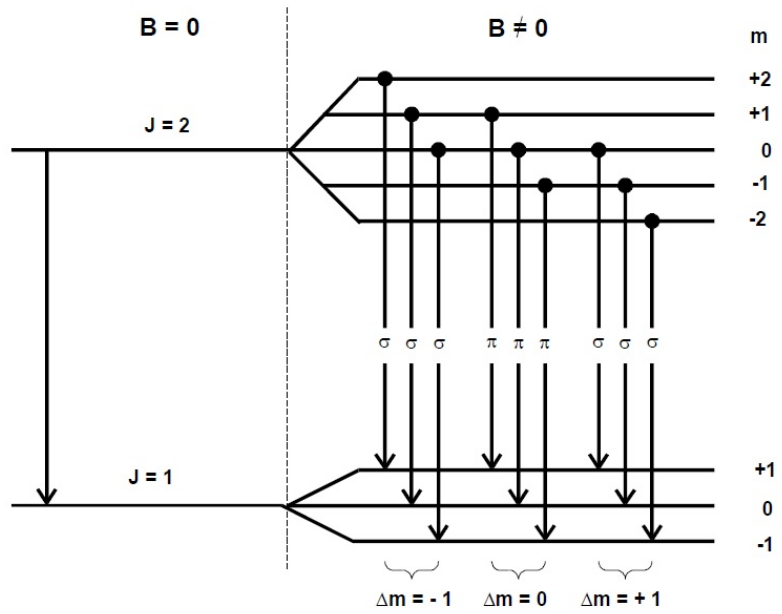
\includegraphics[scale=0.3]{content/normalerzeeman.png}
    \caption{Versuchsaufbau der Messung \cite{alt}.}
    \label{fig:norm}
\end{figure}

\subsection{Anormaler Zeeman-Effekt}

\vspace{-5pt}
\begin{figure}[H]
    \centering
    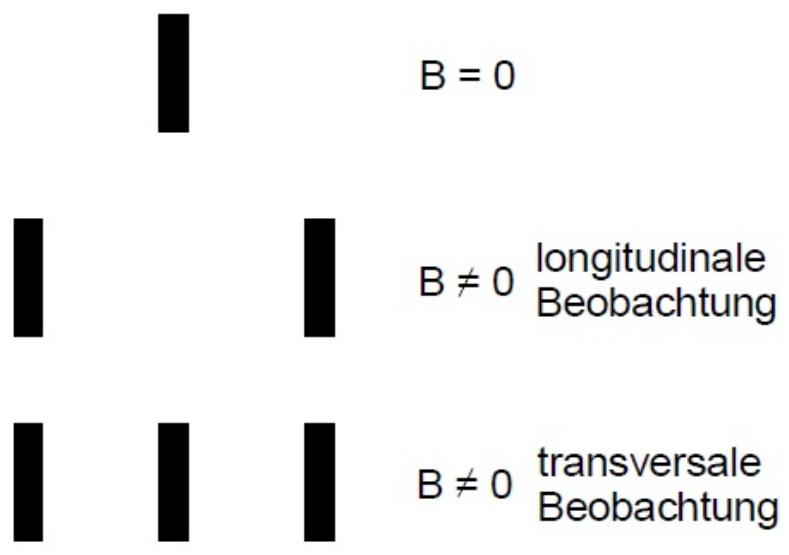
\includegraphics[scale=0.3]{content/polarisation.png}
    \vspace{-10pt}
    \vspace{3pt}
    \caption{Versuchsaufbau der Messung \cite{alt}.}
    \label{fig:pol}
\end{figure}


\vspace{-5pt}
\begin{figure}[H]
    \centering
    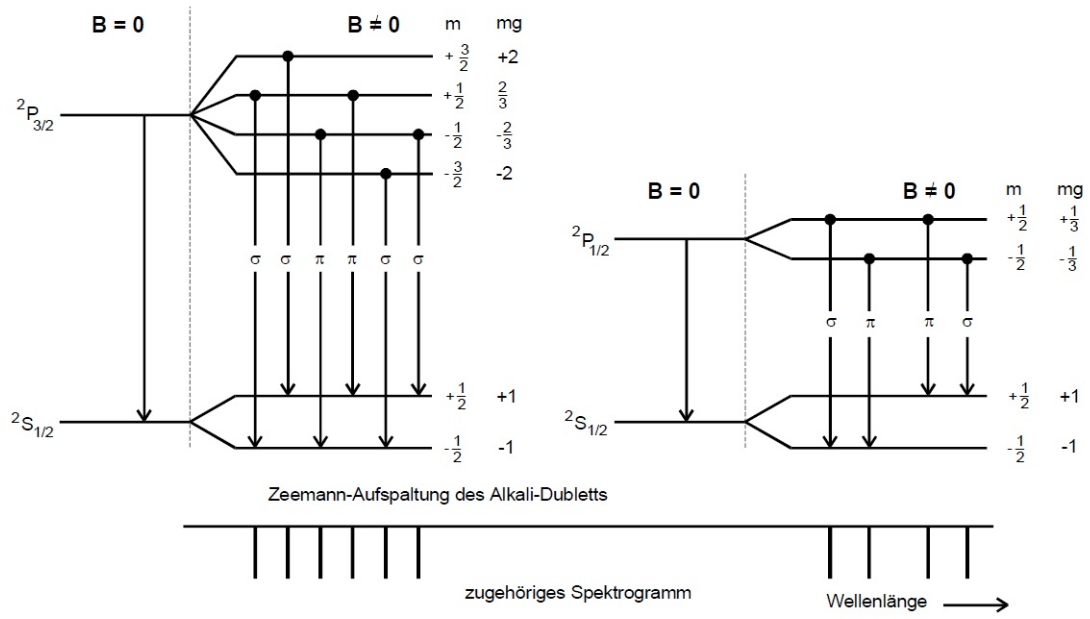
\includegraphics[scale=0.3]{content/anormalerzeeman.png}
    \caption{Versuchsaufbau der Messung \cite{alt}.}
    \label{fig:anorm}
\end{figure}

















